\documentclass[11pt,a4paper,oneside]{report}             % Single-side
%\documentclass[11pt,a4paper,twoside,openright]{report}  % Duplex

%\PassOptionsToPackage{chapternumber=Huordinal}{magyar.ldf}
\usepackage{t1enc}
\usepackage[utf8]{inputenc}
\usepackage{amsmath}
\usepackage{amssymb}
\usepackage{enumerate}
\usepackage[thmmarks]{ntheorem}
\usepackage{graphics}
\usepackage{epsfig}
\usepackage{listings}
\usepackage{color}
%\usepackage{fancyhdr}
\usepackage{lastpage}
\usepackage{anysize}
\usepackage[magyar]{babel}
\usepackage{sectsty}
\usepackage{setspace}  % Ettol a tablazatok, abrak, labjegyzetek maradnak 1-es sorkozzel!
\usepackage[hang]{caption}
\usepackage{hyperref}

%--------------------------------------------------------------------------------------
% Main variables
%--------------------------------------------------------------------------------------
\newcommand{\vikszerzo}{Kovács Ádám}
\newcommand{\vikkonzulens}{Dr.~Recski Gábor}
\newcommand{\vikcim}{Semantic parsing with graph transformations}
\newcommand{\viktanszek}{Department of Automation and Applied Informatics}
\newcommand{\vikdoktipus}{Master's Thesis}
\newcommand{\vikdepartmentr}{Kovács Ádám}

%--------------------------------------------------------------------------------------
% Page layout setup
%--------------------------------------------------------------------------------------
% we need to redefine the pagestyle plain
% another possibility is to use the body of this command without \fancypagestyle
% and use \pagestyle{fancy} but in that case the special pages
% (like the ToC, the References, and the Chapter pages)remain in plane style

\pagestyle{plain}
%\setlength{\parindent}{0pt} % ?ttekinthet?bb, angol nyelv? dokumentumokban jellemz?
%\setlength{\parskip}{8pt plus 3pt minus 3pt} % ?ttekinthet?bb, angol nyelv? dokumentumokban jellemz?
\setlength{\parindent}{12pt} % magyar nyelv? dokumentumokban jellemz?
\setlength{\parskip}{0pt}    % magyar nyelv? dokumentumokban jellemz?

\marginsize{35mm}{25mm}{15mm}{15mm} % anysize package
\setcounter{secnumdepth}{0}
\sectionfont{\large\upshape\bfseries}
\setcounter{secnumdepth}{2}
\singlespacing
\frenchspacing

%--------------------------------------------------------------------------------------
%	Setup hyperref package
%--------------------------------------------------------------------------------------
\hypersetup{
    bookmarks=true,            % show bookmarks bar?
    unicode=false,             % non-Latin characters in Acrobat?s bookmarks
    pdftitle={\vikcim},        % title
    pdfauthor={\vikszerzo},    % author
    pdfsubject={\vikdoktipus}, % subject of the document
    pdfcreator={\vikszerzo},   % creator of the document
    pdfproducer={Producer},    % producer of the document
    pdfkeywords={keywords},    % list of keywords
    pdfnewwindow=true,         % links in new window
    colorlinks=true,           % false: boxed links; true: colored links
    linkcolor=black,           % color of internal links
    citecolor=black,           % color of links to bibliography
    filecolor=black,           % color of file links
    urlcolor=black             % color of external links
}

%--------------------------------------------------------------------------------------
% Set up listings
%--------------------------------------------------------------------------------------
\lstset{
	basicstyle=\scriptsize\ttfamily, % print whole listing small
	keywordstyle=\color{black}\bfseries\underbar, % underlined bold black keywords
	identifierstyle=, 					% nothing happens
	commentstyle=\color{white}, % white comments
	stringstyle=\scriptsize\sffamily, 			% typewriter type for strings
	showstringspaces=false,     % no special string spaces
	aboveskip=3pt,
	belowskip=3pt,
	columns=fixed,
	backgroundcolor=\color{lightgray},
} 		
\def\lstlistingname{lista}	

%--------------------------------------------------------------------------------------
%	Some new commands and declarations
%--------------------------------------------------------------------------------------
\newcommand{\code}[1]{{\upshape\ttfamily\scriptsize\indent #1}}

% define references
\newcommand{\figref}[1]{\ref{fig:#1}.}
\renewcommand{\eqref}[1]{(\ref{eq:#1})}
\newcommand{\listref}[1]{\ref{listing:#1}.}
\newcommand{\sectref}[1]{\ref{sect:#1}}
\newcommand{\tabref}[1]{\ref{tab:#1}.}

\DeclareMathOperator*{\argmax}{arg\,max}
%\DeclareMathOperator*[1]{\floor}{arg\,max}
\DeclareMathOperator{\sign}{sgn}
\DeclareMathOperator{\rot}{rot}
\definecolor{lightgray}{rgb}{0.95,0.95,0.95}

\author{\vikszerzo}
\title{\viktitle}
\includeonly{
	titlepage,%
	declaration,%
	abstract,%
	introduction,%
	Yuanfudao-system, %
	chapter1,%
	chapter2,%
	chapter3,%
	acknowledgement,%
}
%--------------------------------------------------------------------------------------
%	Setup captions
%--------------------------------------------------------------------------------------
\captionsetup[figure]{
%labelsep=none,
%font={footnotesize,it},
%justification=justified,
width=.75\textwidth,
aboveskip=10pt}

\renewcommand{\captionlabelfont}{\small\bf}
\renewcommand{\captionfont}{\footnotesize\it}

%--------------------------------------------------------------------------------------
% Table of contents and the main text
%--------------------------------------------------------------------------------------
\begin{document}
\singlespacing

\pagenumbering{arabic}
\onehalfspacing
%\tableofcontents\vfill
%----------------------------------------------------------------------------
% Abstract in hungarian
%----------------------------------------------------------------------------
\chapter*{Kivonat}\addcontentsline{toc}{chapter}{Kivonat}
%--------------------------------------------------------------------------------------
% semantic parsing, graftranszformacio altalaban
A szemantikai elemzés célja, hogy természetes nyelvi adathoz
készíthessünk szemantikai reprezentációt, így tudjuk modellezni a szöveg jelentését. Ha a nyelvi
jelentést fogalmak irányított gráfjaival reprezentáljuk, ezeket pedig a mondat szintaktikai
szerkezetét reprezentáló fákból kell előállítanunk, akkor a teljes feladat egyetlen komplex gráftranszformációként
definiálható.

%--------------------------------------------------------------------------------------
% machine comprehension
A természetes nyelv szemantikájának reprezentációját ritkán használják közvetlenül a state-of-the art rendszerekben népszerű szemantikai feladatokra, mint a szemantikai hasonlóság mérése, vagy a gépi szövegértés. Ezek a rendszerek többnyire szó embeddingeket használnak a szavak jelentésének ábrázolására.
Ebben a dolgozatban mi gráf reprezentációkat és transzformációkat használunk, mint egyszerű ám hatékony eszközök az oksági viszony felismerésére, valamint leírunk egy módszert a \texttt{4lang} szemantikus elemzőrendszer (Recski:2016) használatára a 2018-as Semeval Task \textit{Machine comprehension using commonsense knowledge} kapcsán. Ez a feladat azt kívánja a résztvevőktől, hogy olyan rendszereket tanítsanak fel, amelyek ki tudják választani a megfelelő választ az egyszerű, több válaszlehetőséget kínáló kérdéseknél rövid eseményleíró szövegek elolvasása után. A tanító és teszt adat az \texttt{MCScript} adathalmaz (Ostermann et al., 2018) részhalmazából lett kinyerve.
A két legjobb rendszer, \texttt{HFL-RC} (Chen et al., 2018) és \texttt{Yuanfudao} egyenként $84,15\%$ és $83,95\%$ pontosságot ért el a teszt adaton.

%--------------------------------------------------------------------------------------
% baseline
Először bemutatunk egy hatékony baselinet ezen a feladaton csupán a szemantikus gráfok és a köztük lévő hasonlóságok felhasználásával. Ezt követően leírjuk a \texttt{Yuanfudao} (Wang et al., 2018) state-of-the art rendszert és az ezzel végzett kísérletezéseinket, amelyek során
%--------------------------------------------------------------------------------------
% rendszer, amivel foglalkoztunk
a baselineunkat extra featureként felhasználva javítottunk a neurális hálón. A rendszer kiválasztása magától értetődő volt, mivel a forráskód nyilvánosan elérhető és már sikeresen alkalmazott tudás alapú reprezentációt a szópárok közötti szemantikai kapcsolatokra, a \textit{ConceptNet}et.
Eredményeink azt mutatják, hogy ezzel a módosítással $0,5\%$ százalékpont növekedés érhető el és a \textit{ConceptNet} helyettesíthető a mi szemantikus modellünkkel.
\vfill

%----------------------------------------------------------------------------
% Abstract in english
%----------------------------------------------------------------------------
\chapter*{Abstract}\addcontentsline{toc}{chapter}{Abstract}
%--------------------------------------------------------------------------------------
% semantic parsing, graftranszformacio altalaban
The main task of semantic parsing is to automatically build semantic representation from the input, so we can model the meaning
of raw texts. If we model meaning as directed graphs of concept and we can build them from syntax trees that represent the structure of 
sentences, then we can define the whole process as one complex graph transformation.

%--------------------------------------------------------------------------------------
% machine comprehension
Representations of natural language semantics are rarely used explicitly in state-of-the art systems for popular semantics tasks such as measuring semantic similarity or machine comprehension. These systems mostly use word embeddings as representation of word meaning.

In this paper we use graphical representations and transformations as simple but powerful tools for recognizing entailment and we describe a method using semantic parsing system \texttt{4lang} (Recski:2016) and applying it on the 2018 Semeval Task \textit{Machine comprehension using commonsense knowledge}. This task requires participants to train systems that can choose the correct answer to simple multiple choice questions based on short passages describing simple chains of events. Data for both training and testing is extracted from the \texttt{MCScript} dataset (Ostermann et al., 2018). The top two systems, \texttt{HFL-RC} (Chen et al., 2018) and \texttt{Yuanfudao} achieved accuracy scores of $84.15\%$ and $83.95\%$ on the test data, respectively.

%--------------------------------------------------------------------------------------
% baseline
First we will present a strong baseline on this task using only semantic graphs and similarities among them, followed by 
a description of a state-of-the art system \texttt{Yuanfudao} (Wang et al., 2018) and our experiments with it where
%--------------------------------------------------------------------------------------
% rendszer, amivel foglalkoztunk
we used our baseline as an extra feature for improving the neural network. The choice of the system was obvious, because the source code is publicly available and it already employs successfully a knowledge base representing semantic relationships among pairs of words, \textit{ConceptNet}.
Our results suggest that these features achieve a .5 percentage point improvement, and the \textit{ConceptNet} could be replaced by our semantic model.
\vfill


\chapter{Introduction}
\label{chap:Introdu}
%----------------------------------------------------------------------------
\section{Natural Language Processing}
While computers can be easily programmed to understand structured data, such as tables and spreadsheets, it can be rather challenging for them
to understand human communication. Because there is a vast difference in the magnitude of the unstructured data compared to the structured ones, there is a high demand
for tools, that can deal with raw text. Thats where NLP comes in. It contains high variety of tools, that we have to use, when we need to deal with natural input.

Every day, we come into contact with human communication, we say a lot of words to other people, and they try to interpret them even when the context of the saying 
isn't necesseraily complete. The listeners can use their common knowledge to fill the needed information. We resolve ambiguities, misunderstanding, and can even understand words 
we have never heard before just from the context of the communication.
Even though these tasks are trivial for us, for a computer it can be really hard.

%--------------------------------------------------------------------------------------
% egyszer� multtol jelenig bevezeto
The interest in NLP research began in the 1950s, the early phase was mainly focused on MT (Machine Translation), because after the World War II, people
recognised the importance of the translation from one language to another, and hoped to do it automatically.
However MT is still a very difficult nowadays, so these researches discovered early the main challenges of the syntactic and semantic parsing.
As time passed, researches embraced new areas of NLP as more advanced technology and knowledge became available. Now that we live in a world where
computers and smartphones, collecting data became incredibly easy, as a result, statistical NLP drew attention because these models thrive off big data, but one cannot ignore 
simple rule based methods, which can also be a very powerful method, especially using them as a hybrid model with statistical methods.
%--------------------------------------------------------------------------------------
% r�vid nlp pipeline

Building NLP applications requires many levels of analysis.
The typical pipeline structured as follows:
\begin{itemize}
	\item First we need to tokenize our input text, which means breaking up the text into meaningful elements, especially into words
	\item After we tokenized our text, we need word analysis called \texttt{morphology}, which is concerned with the structure of words.
	\item Part of speech explains how a word is used in a sentence, and tagging is a process marking words to its particular part of speech.
	\item The main task of syntactic parsing is to analyze the grammatical structure of a sentence. Given a set of words, a parser forms units (subjects, verbs, etc..) according to some grammatical formalism.
	There are two main type of syntactic parsers:
	\begin{itemize}
		\item Consituency parsers produce trees, that represents the grammatical structure.
		\item Dependency parsers are the more popular nowadays. They represent the structure of a sentence as a dependency tree.
	\end{itemize}
	\item At this point we have various ways to analyze a text, but without modeling its \texttt{meaning}. Semantic is the study of meaning, and semantic parsing is a task to find a representation and assign it to the text. This task will be the main topic of my work.
\end{itemize}
\chapter{Yuanfudao system}
\label{chap:yuanfudao}
On the 2018 Semeval Task \textit{Machine comprehension using commonsense knowledge} competition the \texttt{Yuanfudao} \cite{Wang:2018} system reached second place with $83.95\%$ accuracy on the test data.

% Yuanfudao introduction
\section{The original system}

The \texttt{Yuanfudao} system implements a Three-way Attentive Network (TriAN), an ensemble of three LSTMs augmented with various attention mechanisms, to model for each question interactions between question, possible answers, and the passage that may or may not contain the correct answer to the question.

The system was implemented using python programming language and the \texttt{pytorch} package for the implementation of the neural network. The source code is available on Github\footnote{\url{https://github.com/intfloat/commonsense-rc}}.

% Yuanfudao preprocess

\subsection{Preprocessing}
This system processes the input data as follows:

\begin{enumerate}
	\item Using the \texttt{spacy} package's tokenizer function it generates the part of speech (pos) tag, named entity recognition (ner) tag and the lemma for each word in the passage, and the pos tags of the questions.
	\item It assigns a number representation and an offset for each word in the passage, questions and answers.
	\item It also saves the ids of the passages, questions and answers and whether the answer was correct.
	\item The preprocessor finds the words and lemmas in the questions and answers, that also occurred in the passage's word and lemma list. 
	\item It stores each word's frequency using the \texttt{wikiwords} library.
	\item It  establishes the \textit{ConceptNet} relation between the words of the passage and question and also between the words of the passage and answer.
	\item The preprocessor saves all this data to their respective json files.
\end{enumerate}


\paragraph*{Conceptnet} \cite{Speer:2017} \\

\textit{ConceptNet} plays a major part of the \texttt{Yuanfudao} system, as it was shown in the original paper \cite{Wang:2018}. This is a metric  used to show the possible relationship between two words. These relations could be "RelatedTo", "IsA", "Synonym", "PartOf" etc. 

The \textit{ConceptNet} itself is a large graph of general knowledge that has shown to be affective at determining word relations.

The preprocessor compares the words in the passage with the words in the "query" (question or answer) using \textit{ConceptNet} and stores only one of the matches per word, if there were any.

% System description

\subsection{System description}

An overview of the original system is reproduced in Figure~\ref{fig:dnn}.
\begin{figure}[h!]
	\centering
	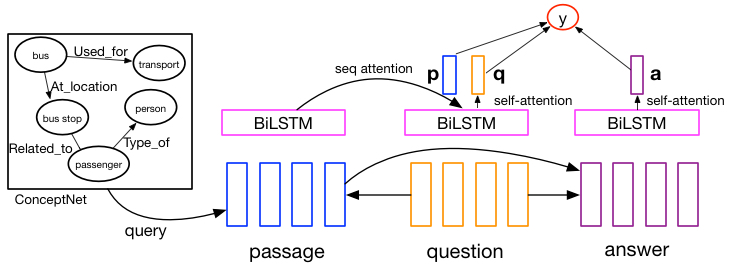
\includegraphics[scale=0.5]{TriAN.jpg}
	\caption{Structure of the original network \cite{Wang:2018}}
	\label{fig:dnn}
\end{figure}

This system is a deep learning neural network consisting of embeddings, recurrent neural networks and attention mechanisms.

First the inputs generated in the preprocessing phase go through three embedding layers, each corresponding to the passage, question and answer respectively. There are also pos-embedding, ner-embedding and rel-embedding layers. The pos-embedding gets the passage's and the question's pos tags as its input, the ner-embedding layer gets the passage's ner-tags and the relation-embedding gets the relationship vectors generated using the \textit{ConceptNet}. This input embedding layer is shown in Figure~\ref{fig:embedding}.
\begin{figure}[h!]
	\centering
	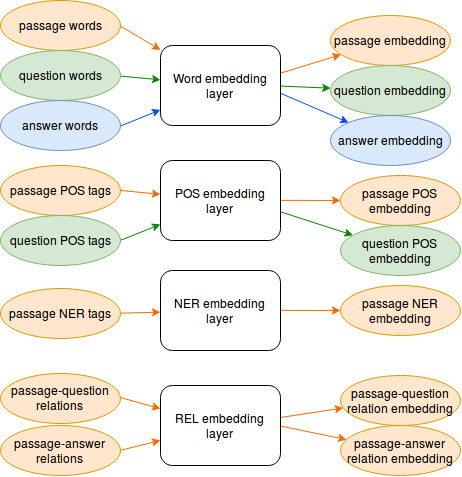
\includegraphics[scale=0.5]{TriAN_embeddings.jpg}
	\caption{Structure of the input embedding layers.}
	\label{fig:embedding}
\end{figure}

The word embeddings' outputs are paired up (passage-question, answer-question, answer-passage) and go through a so called \textit{sequence attention matching layer}.
The sequence attention matching layer at its core uses the bmm function in \texttt{pytorch} which performs a batch matrix-matrix product of the input matrices.
This way it "matches" the two inputs together. This is shown in Figure~\ref{fig:attention_match}.
\begin{figure}[h!]
	\centering
	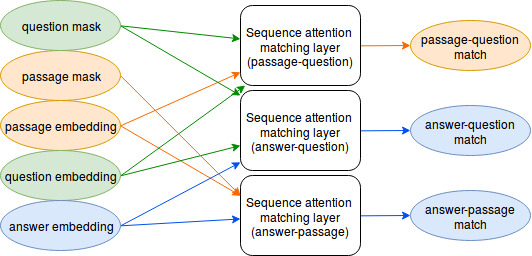
\includegraphics[scale=0.5]{TriAN_attention_match.jpg}
	\caption{Structure of the \textit{sequence attention matching layers}.}
	\label{fig:attention_match}
\end{figure}

The system uses dropouts after the embedding and sequence attention matching layer layers to avoid over-fitting.

These layers are followed by three \textit{stacked bidirectional RNN layer}, each corresponding to the passage, question and answer respectively. It differs from the standard bidirectional RNN layer in one aspect: it can concatenate the hidden states of the RNN. By default the type of the RNN is LSTM, but it can also be GRU. Their inputs are sort of self explanatory. The passage's stacked bidirectional RNN layer gets the passage's word embedding layer, the output of the sequence attention matching layer for the passage-question input pair, the passage's pos- and ner-embedding layers, the word frequency tensor created with the \texttt{wikiword} library, and the two relation-embedding layer's output. The question's stacked bidirectional RNN layer expects the question's word and pos-embedding outputs on its input. The answer's stacked bidirectional RNN layer's inputs are the answer's word embedding output and  the output of the sequence attention matching layer for the answer-question and the answer-question input pairs. These RNN layers are shown in the Figure~\ref{fig:rnn}.
\begin{figure}[h!]
	\centering
	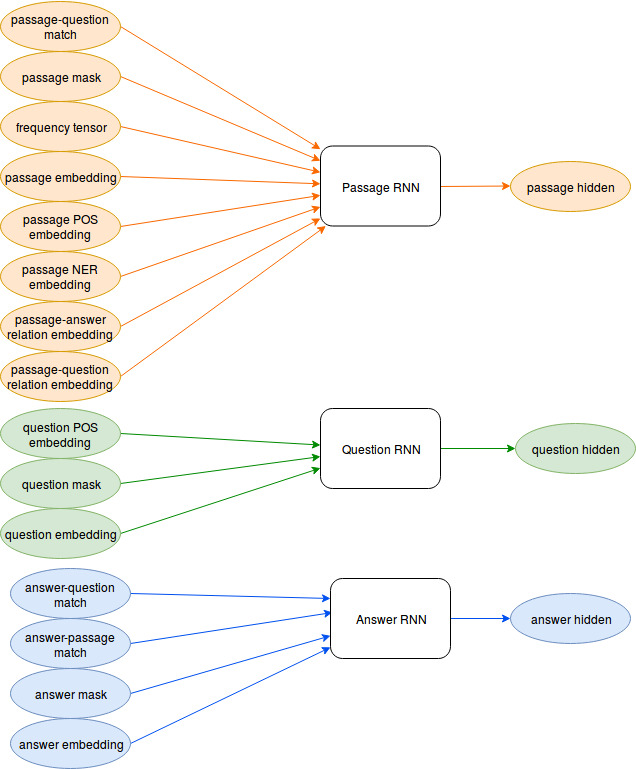
\includegraphics[scale=0.4]{TriAN_rnn.jpg}
	\caption{Structure of the \textit{stacked bidirectional RNN layers}.}
	\label{fig:rnn}
\end{figure}
This layer implicitly uses a dropout rate for regularization.

The question's and the answer's stacked bidirectional RNN layer's outputs are used in two \textit{linear sequence attention layers}, or better known as \textit{self-attention layers over a sequence} for the question and the answer respectively. This layer is basically a linear layer slightly modified, so the infinite outputs are masked and it uses a softmax function at its output.

The passage's stacked bidirectional RNN layer's output is used differently. The system passes it and the question's \textit{stacked bidirectional RNN layer's} output to a \textit{bilinear sequence attention layer}, which is similarly to the sequence attention matching layer uses the bmm function as its core function.

The two linear sequence attention layer's and the bilinear sequence attention layer's output is passed through a weighted averaging function with their respective stacked bidirectional RNN layer's output. This part of the network is shown in Figure~\ref{fig:sequence_attention}.
\begin{figure}[h!]
	\centering
	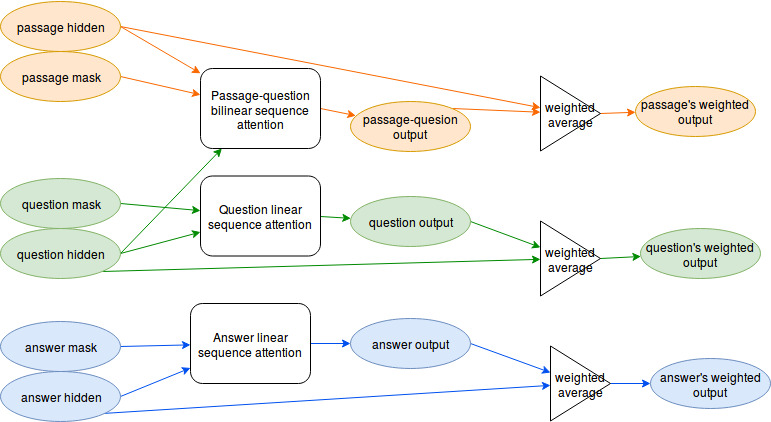
\includegraphics[scale=0.5]{TriAN_sequence_attention.jpg}
	\caption{Structure of the sequence attention layer\\and the following weighted average function.}
	\label{fig:sequence_attention}
\end{figure}

The averaged passage output is passed though a \textit{linear feed forward layer} than multiplied by the answer's averaged output. The question's averaged output is passed though an other linear feed forward layer than multiplied by the answer's averaged output. At the end its all summed and sigmoid function used at its output. The output in this case is whether the answer was correct to the given question or not. This last section is at Figure~\ref{fig:output}.
\begin{figure}[!htb]
	\centering
	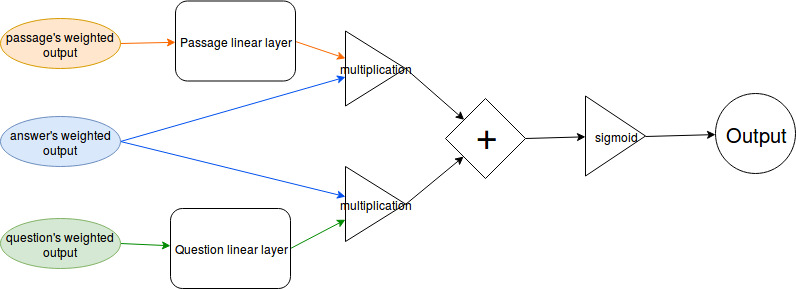
\includegraphics[scale=0.5]{TriAN_output.jpg}
	\caption{Structure of the output of the network.}
	\label{fig:output}
\end{figure}


\subsection{Parameters}
\begin{minipage}{\textwidth}
The \texttt{Yuanfudao} system has these following command line arguments:
\begin{itemize}
	\item \textbf{GPU}: the training of the system can be done on GPU which is much faster than training it on CPU
	\item \textbf{using cuda}: \texttt{pytorch} can support CUDA for parallelization. The system uses CUDA by default.
	\item \textbf{optimizer}: the optimizer function can be adamax (default) or SGD
	\item \textbf{RNN type}: the RNN used by the system can be LSTM or GRU
	\item \textbf{dropout rate}: there are separate dropout rates for embeddings and RNNs
	\item \textbf{embedding dimension}: each embedding dimension in the system can be manually set
	\item \textbf{gradient clipping}: the gradient clipping threshold can be set
	\item \textbf{epoch}
	\item \textbf{learning rate}
	\item \textbf{batch size}
	\item \textbf{random seed}
	\item other parameters related to input handling, RNN settings and testing
\end{itemize}
You can read about the deep learning related arguments and their functions in Chapter \ref{chap:deep}.
\end{minipage}

\subsection{Learning curve}
\begin{minipage}{\linewidth}
Without the recommended pretraining (Figure~\ref{fig:learning_curve}):
\begin{itemize}
	\item Max dev accuracy: $82.7\%$ reached in the 26th epoch
	\item Train accuracy: $97.7\%$ reached in the 26th epoch
	\item Max train accuracy: $99.8\%$ reached in the 50th epoch
	\item Last dev accuracy: $81.9\%$
	\item Average dev accuracy after ten epochs: $81.9\%$
\end{itemize}
\end{minipage}
\begin{figure}[!htb]
	\centering
	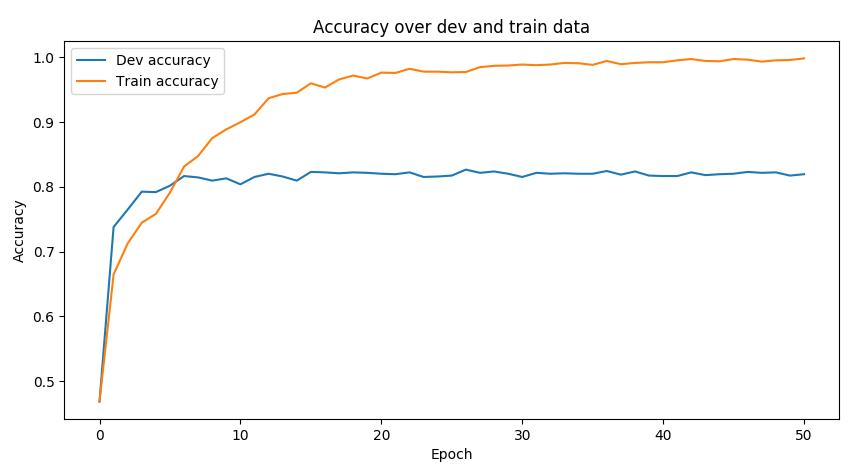
\includegraphics[scale=0.5]{learning_curve.jpg}
	\caption{Learning curve without pretraining.}
	\label{fig:learning_curve}
\end{figure}

\begin{minipage}{\linewidth}
With the recommended pretraining(Figure~\ref{fig:learning_curve2}):
\begin{itemize}
	\item Max dev accuracy: $82.5\%$ reached in the 38th epoch
	\item Train accuracy: $99\%$ reached in the 38th epoch
	\item Max train accuracy: $99.7\%$ reached in the 50th epoch
	\item Last dev accuracy: $82.2\%$
	\item Average dev accuracy after ten epochs: $81.9\%$
\end{itemize}
\end{minipage}
\begin{figure}[!htb]
	\centering
	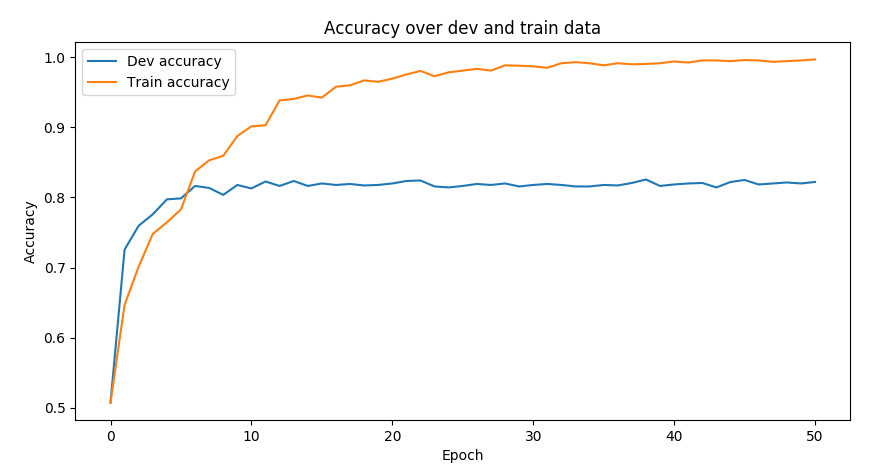
\includegraphics[scale=0.5]{learning_curve2.jpg}
	\caption{Learning curve with pretraining.}
	\label{fig:learning_curve2}
\end{figure}

As you can see there is no significant difference between the learning curve with or without pretraining.

\section{Modifications}
Our modifications are available on Github\footnote{\url{https://github.com/GKingA/commonsense-rc}}.

We modified the preprocessing part of the system to incorporate the similarity calculating method from Chapter ~\ref{chap:comprehension}. The most straightforward way of incorporating our metric into the system is by creating vectors similar to those representing \textit{ConceptNet} relations between words of a passage and words in each answer candidate. Since these vectors represent
word-to-word relationships, we measure the support between pairs of \texttt{4lang} definition graphs, and for each word in the passage we take the maximum support score over all words of the answer candidate. Elements of a vector for a passage $P$ and a possible answer $A$ are hence defined as:

\[S^{(P, A)}_i = \max_{A_j \in A} S(P_i, A_j)\]

Elements of a vector for a passage $P$ and a question $Q$ are defined as:

\[S^{(P, Q)}_i = \max_{Q_j \in Q} S(P_i, Q_j)\]

Elements of a vector for a question $Q$ and an answer $A$ are defined as:

\[S^{(Q, A)}_i = \max_{A_j \in A} S(Q_i, A_j)\]

We used these new input vectors as the input of a new \texttt{4lang} embedding layer that functions similarly to the other embedding layers. It is shown at Figure~\ref{fig:4lang_embedding}. The input of this layer is 101 dimensional, since the similarities are on a scale to 0 to 100.

\begin{figure}[h!]
	\centering
	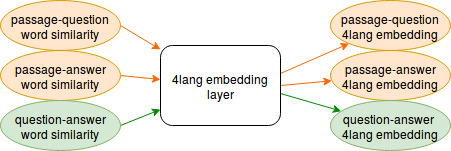
\includegraphics[scale=0.5]{4lang_embedding.jpg}
	\caption{\texttt{4lang} embedding layer.}
	\label{fig:4lang_embedding}
\end{figure}

The outputs of this layer is passed to the RNN layers. This is depicted at Figure~\ref{fig:rnn_4lang}.

\begin{figure}[h!]
	\centering
	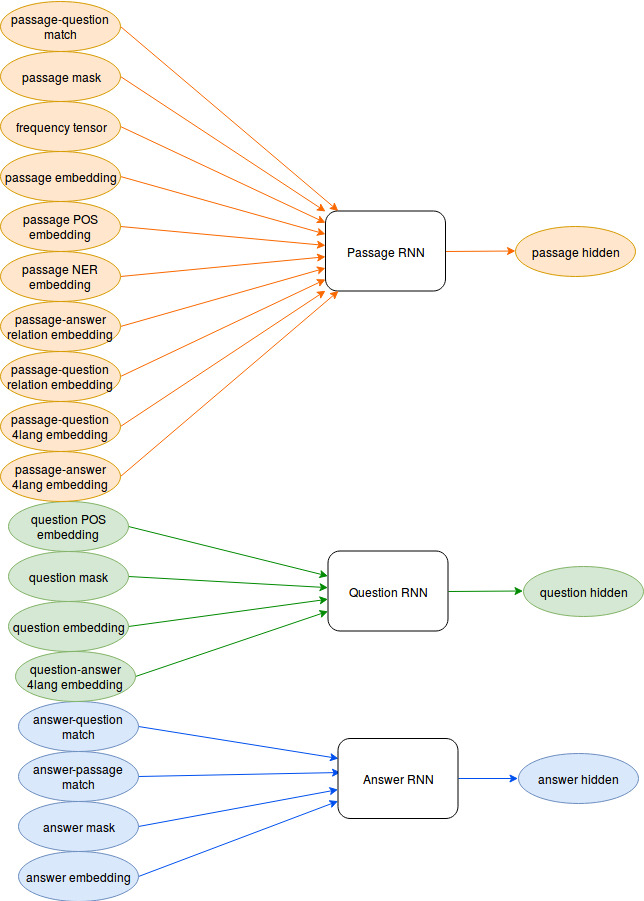
\includegraphics[scale=0.4]{TriAN_rnn_with_4lang.jpg}
	\caption{Structure of the modified \textit{stacked bidirectional RNN layers}.}
	\label{fig:rnn_4lang}
\end{figure}

Since we also wanted to see how the system changes if we replace \textit{ConceptNet} relations with our metric, we also trained systems without \textit{ConceptNet} rel-embeddings.

\FloatBarrier

\section{The results}
The original \texttt{Yuanfudao} \cite{Wang:2018} publication said its system was able to reach $83.95\%$ accuracy on the test data. We were only able to reproduce a $80.3\%$ accuracy on the test set and $82.5\%$ on the development set with the recommended pretraining on the \texttt{RACE} \cite{Lai:2017} dataset. We will take these results as our bases of the comparison.

We tested our model by turning on and off the usage of \textit{ConceptNet} and \texttt{4lang}. There were 4 combinations: using neither, just \textit{ConceptNet}, just \texttt{4lang} and both.

\begin{table}[h!]
	\centering
	\begin{tabular}{ | l | c | r | }
		\hline
		model & dev & test \\ \hline \hline
		pretrained TriAN, no ConceptNet & 83.7\% & 81.9\% \\ \hline
		pretrained TriAN, with ConceptNet & 82.5\% & 80.3\% \\ \hline
		pretrained TriAN, with 4lang & 84.2\% & 81.5\% \\ \hline
		\textbf{pretrained TriAN, with both} & \textbf{83.4\%} & \textbf{82.9\%} \\ \hline
		TriAN, no ConceptNet & 82.8\% & 80.2\% \\ \hline
		TriAN, with ConceptNet & 82.7\% & 80.5\% \\ \hline
		TriAN, with 4lang & 83.2\% & 80.9\% \\ \hline
		TriAN, with both & 83.1\% & 80.8\% \\ \hline
	\end{tabular}
	\caption{Effect of \texttt{4lang} and \texttt{ConceptNet} on results}
	\label{tabl:res}
\end{table}

It is evident that without pretraining the Yuanfudao system performs best if we use the relation scores calculated from \texttt{4lang} graphs instead of the \textit{ConceptNet} relationships.
After pretraining the network on the \texttt{RACE} dataset the results show that using both of the relation metric is most beneficial.

%\listoffigures\addcontentsline{toc}{chapter}{?br?k jegyz?ke}
%\listoftables\addcontentsline{toc}{chapter}{T?bl?zatok jegyz?ke}


%\bibliography{mybib}
%\addcontentsline{toc}{chapter}{Irodalomjegyz?k}
\bibliographystyle{plain}

\label{page:last}
\end{document}

